\section{Results}
\newcommand{\FinalWarningScenarios}{81}
\newcommand{\FinalTrueWarnings}{10}
\newcommand{\FinalConservativeWarnings}{32}
\newcommand{\FinalSimultaneousWarnings}{39}
\newcommand{\FinalRobustWarnings}{4}
\newcommand{\FinalMSevenMisses}{20}
\newcommand{\FinalRhoJump}{406.0978}
\newcommand{\FinalGTwo}{4.21649}
\newcommand{\FinalGInf}{5.16703}
\newcommand{\FinalGradientValid}{0}
\newcommand{\FinalFallback}{1}

% Auto-generated from immutable Phase 2M-FOLLOWUP logs; do not edit numerically.
\newcommand{\FollowupScenarioCount}{81}
\newcommand{\FollowupTrueWarningCount}{10}
\newcommand{\FollowupConservativeWarningCount}{32}
\newcommand{\FollowupSimultaneousWarningCount}{39}
\newcommand{\FollowupMissedWarningCount}{0}
\newcommand{\FollowupRobustTrueWarningCount}{4}
\newcommand{\FollowupMaxGTwo}{4.21649}
\newcommand{\FollowupMaxGInf}{5.16703}


\subsection{Model-Based Feasibility and Allocation Evidence}
The registered M1 288-state sweep evaluates signed-reserve sensitivity: dual braking increases reserve at 192/288 matched points, while both formulations are feasible at 270/288 points. A separate $25\times51$ initial-state boundary follow-up evaluates feasible-domain expansion at 15~m/s on a 10\% downgrade. Among 1,275 temperature-gap states spanning 365--461~K and 15--90~m, 1,071 are friction-only feasible, 1,114 are dual feasible, and 43 are feasible only with dual braking (Fig.~\ref{fig:feasibility-frontier}). At 413~K/24~m, reserves are $-1.466$ versus $0.027$, limited by thermal and realized-force bounds. This is one-step domain expansion, not recursive feasibility.

\begin{figure*}[t]
\centering
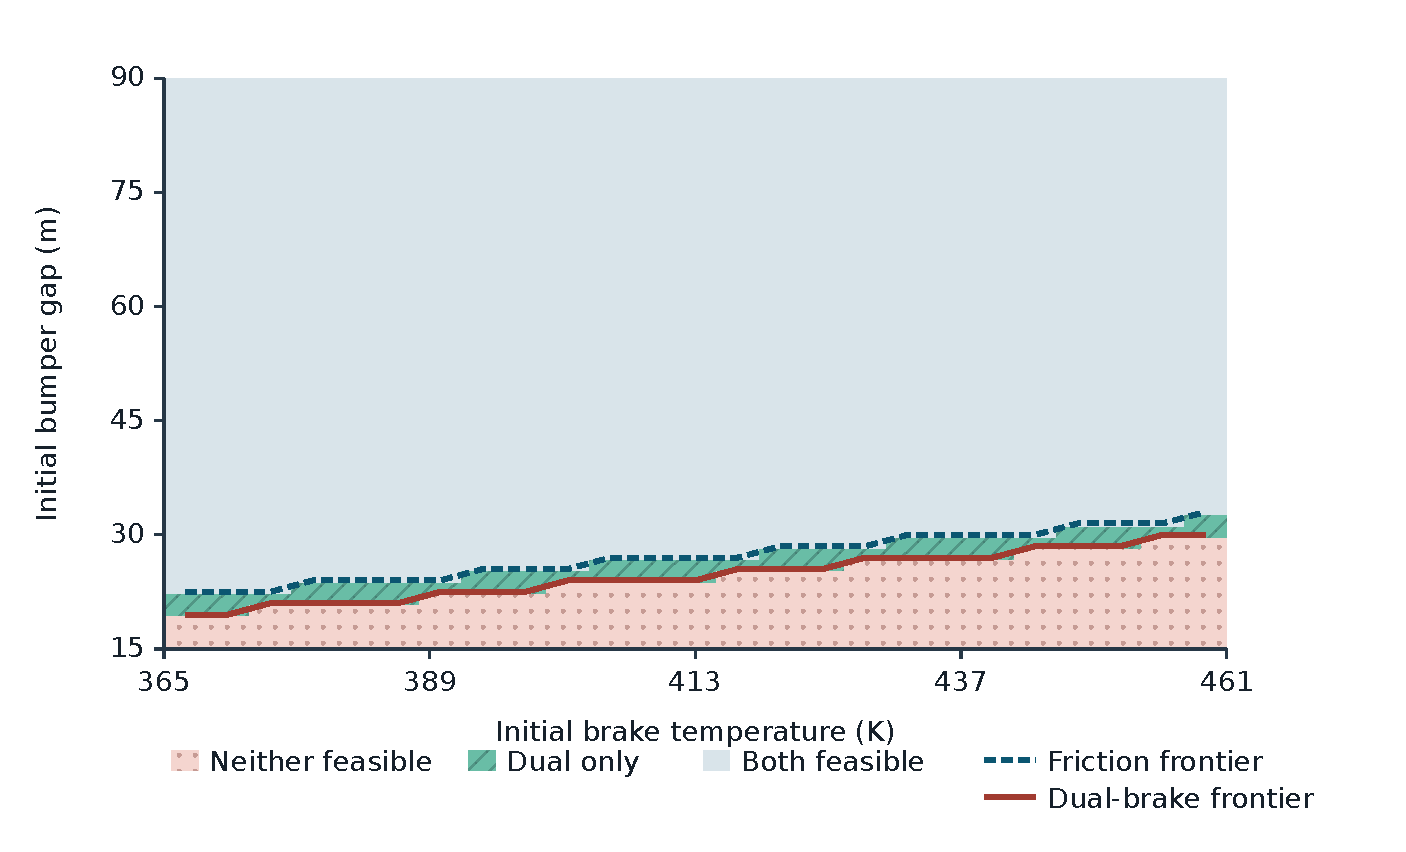
\includegraphics[width=.9\textwidth]{../generated/submission_revision/figures/feasibility_frontier.pdf}
\caption{Initial-command feasibility in the separate 1,275-state boundary follow-up at 15~m/s on a 10\% downgrade. Color and pattern classify the hard set by temperature and gap; dashed/solid curves are friction-only/dual-brake zero-reserve boundaries. The green band is dual-only feasible.}
\label{fig:feasibility-frontier}
\end{figure*}

All four M2 strategies have negative minimum $\rho$ (Table~\ref{tab:phase2m-controller}), so none is universally safe. Allocation changes energy, tracking, and temperature without identifying a learning advantage. M3 loses the certificate earlier as initial temperature nears $T_{\rm crit}$ (Table~\ref{tab:final-model-evidence}).

Across three matched 100-step, three-truck ablations, both supervisors have zero certificate losses on ordinary/hot descents and six in leader braking; pairwise minima are 0.059, 0.023, and $-2.076$. Predictive/upstream triggering adds 156, 300, and 294 anticipatory truck-samples but no observed loss reduction.

\begin{table*}[!t]
\centering
\caption{Selected model-based evidence from the Phase 2M analysis.}
\label{tab:final-model-evidence}
\normalsize
\begin{tabular}{@{}lp{.35\textwidth}lp{.28\textwidth}@{}}
\toprule
Study & Quantity & Result & Interpretation \\
\midrule
M1 & Dual/friction feasible points & 270/288; 270/288 & No count increase in M1 sweep \\
M1 & Positive dual-reserve gain & 192/288 & Margin improvement only \\
M3 & Certificate loss at $T_0=413.7$ K & 16.4 s & collision\_demand \\
M3 & Certificate loss at $T_0=453.7$ K & 11 s & collision\_demand \\
M3 & Certificate loss at $T_0=461.7$ K & 10 s & collision\_demand \\
\bottomrule
\end{tabular}
\end{table*}

\begin{table*}[!t]
\centering
\caption{Matched long-descent deterministic controller comparison; method names abbreviate source-code identifiers.}
\label{tab:phase2m-controller}
\normalsize
\begin{tabular}{@{}lrrrrr@{}}
\hline
Method & Peak $T$ (K) & Min. $\rho$ & $E_f$ (MJ) & $E_a$ (MJ) & Speed RMSE (m/s) \\
\hline
Aux.-first & 458.81 & -28.532 & 12.265 & 25.978 & 2.8775 \\
Fric.-first & 458.8 & -10.141 & 13.233 & 24.796 & 2.3195 \\
Fric.-only & 364.36 & -364.1 & 1.1293 & 0 & 15.938 \\
Dual QP & 458.83 & -17.98 & 12.812 & 25.258 & 2.5585 \\
\hline
\end{tabular}
\end{table*}


\subsection{Predictive, Robustness, Communication, and Low-Speed Evidence}
M4 has no predictive or instantaneous crossing and is inconclusive. M5 verifies prefix-horizon monotonicity; longer horizons can lower numerical reserve (Table~\ref{tab:phase2m-predictive}).

\begin{table*}[!t]
\centering
\caption{Predictive-monitor metrics; dashes denote no crossing, and ``yes'' verifies M5 prefix monotonicity.}
\label{tab:phase2m-predictive}
\normalsize
\begin{tabular}{@{}lrrrrrp{.20\textwidth}@{}}
\hline
Case & Trigger (s) & Boundary (s) & Warning (s) & Vehicle & Step & Component / status \\
\hline
M4 & -- & -- & -- & 1 & 3 & friction interval \\
M5 $H=1$ & -- & -- & -- & -- & -- & yes \\
M5 $H=3$ & -- & -- & -- & -- & -- & yes \\
M5 $H=5$ & 0 & -- & -- & -- & -- & yes \\
M5 $H=10$ & 0 & -- & -- & -- & -- & yes \\
\hline
\end{tabular}
\end{table*}


Among \FollowupScenarioCount{} boundary approaches are \FollowupTrueWarningCount{} isolated early warnings, \FollowupConservativeWarningCount{} nonisolated warnings, and \FollowupSimultaneousWarningCount{} simultaneous crossings; only \FollowupRobustTrueWarningCount{} satisfy the strict adjacent-grid/finite-margin rule (Fig.~\ref{fig:predictive-examples}). At all 32,849 stored numerically positive predictive vehicle-samples, concurrent $\rho_i\ge0$ (minimum 0). This checks implementation consistency, not sound enclosure: the tube check samples 5,000 states, and negative predictions remain inconclusive warnings.

\begin{figure*}[t]
\centering
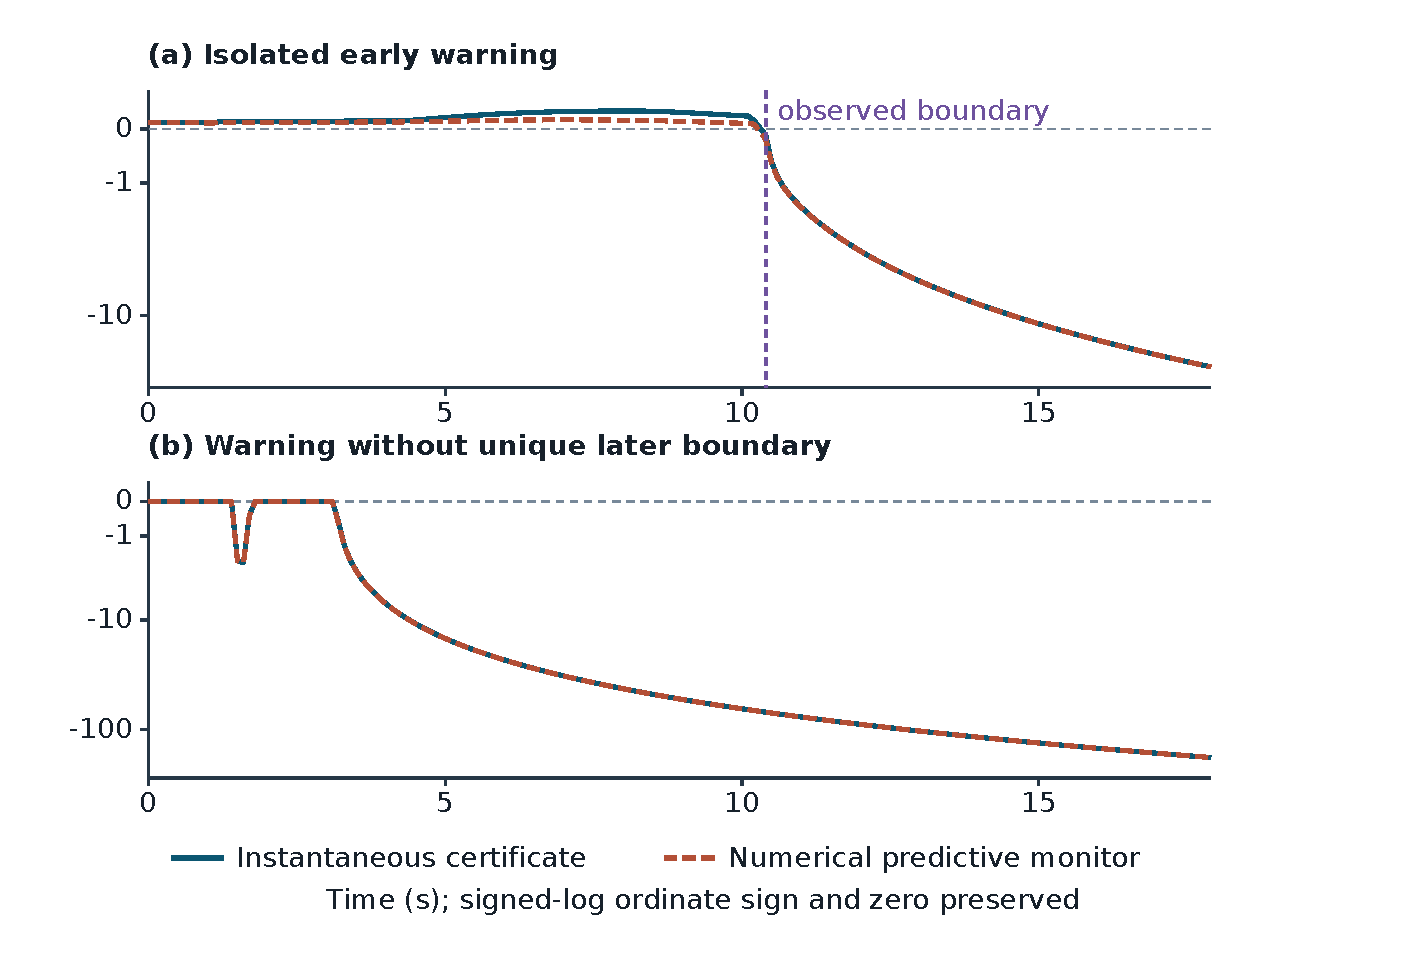
\includegraphics[width=.9\textwidth]{../generated/submission_revision/figures/predictive_examples.pdf}
\caption{Follower-1 instantaneous certificate $\rho_i$ and numerical predictive monitor $\widehat{\rho}_{i,k}^{H}$: isolated early warning (top) and nonisolated warning (bottom). Signed-log scaling preserves zero; these model-based traces are not verified reachable-set bounds.}
\label{fig:predictive-examples}
\end{figure*}

M6 includes one endpoint certificate loss and losses in 3/20 joint design samples. These deterministic samples are not a physical probability law or reliability estimate; complete rows are archived.

A 300-point stratified design varies bounded mass, friction lag, cooling, force limit, auxiliary capacity, and fade-temperature offset near 413~K/24~m. It yields 133 nonnegative initial reserves (range $-1.505$ to 0.059); collision demand limits 172 points and the auxiliary interval 128. These are sensitivity, not failure-probability, results. Zero-width declared intervals fix thermal capacity and auxiliary lag.

M7 shows stale fleet awareness: head-truck mean absolute error against the centralized oracle rises from $3.1\times10^{-6}$ at zero delay to 0.027, 0.055, and 0.078 at 100, 200, and 300~ms. Nominal 50/100~ms delays coincide under 100-ms sampled consumption. Critical-vehicle agreement falls from 1.00 to 0.62, 0.64, 0.62; missed/false triggers are 9/8, 7/10, 6/11, not monotone despite rising mean error. Bounded-delay and stale-message cases each reach 1.118 mean head gap and 112 false triggers (Fig.~\ref{fig:communication}). Non-head vehicles aggregate only their upstream subchain, lowering vehicle-level agreement even at zero delay.

\begin{figure*}[t]
\centering
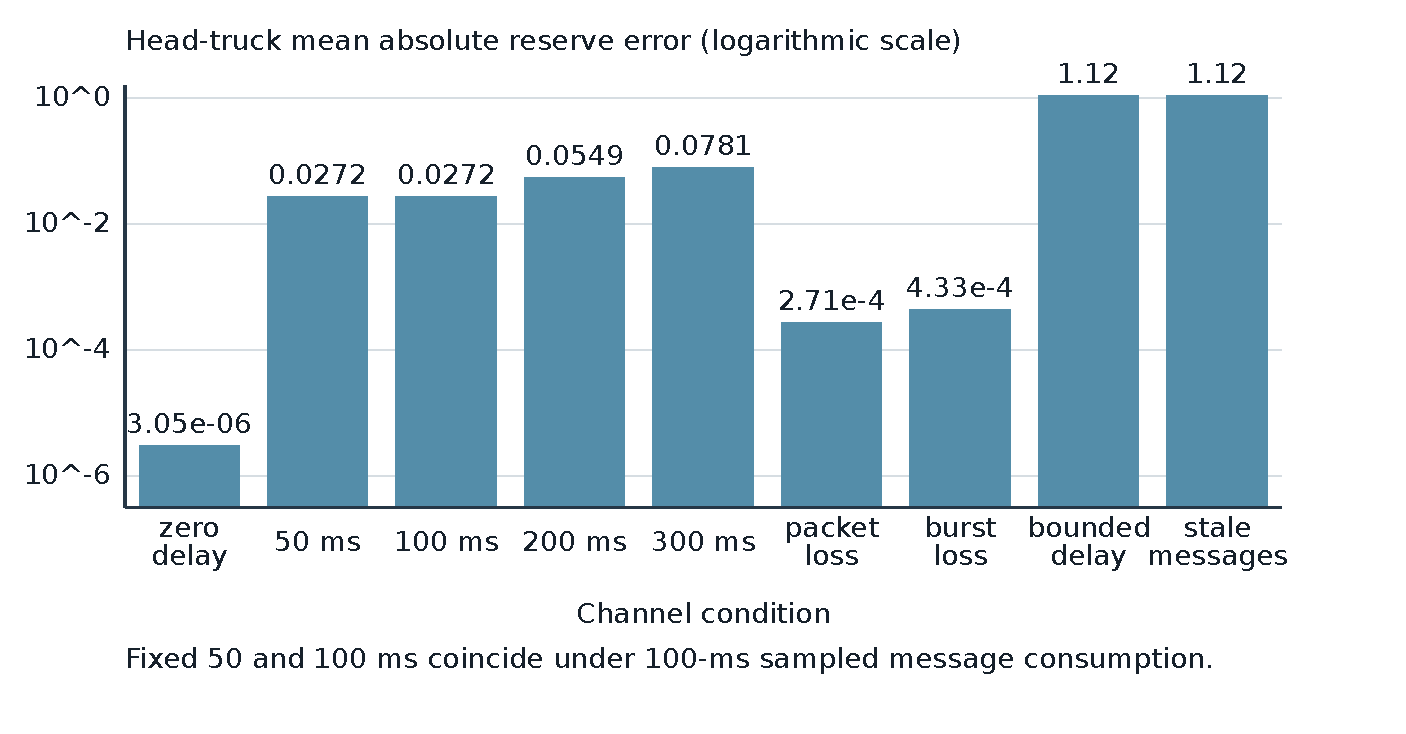
\includegraphics[width=.9\textwidth]{../generated/submission_revision/figures/communication_age.pdf}
\caption{Head-truck age-aware reserve error against the instantaneous oracle under delay/loss/staleness (log scale; 120 samples per case). The 50/100-ms cases coincide under 100-ms sampled consumption.}
\label{fig:communication}
\end{figure*}

M8 rows remain finite but the hot-brake reserve jumps at $v_\epsilon$: ZOH and high-order barrier branches are distinct sufficient conditions, so normalized reserves need not match. Smoothing would compromise exact feasibility; the hard switch remains, without implying physical discontinuity. The supervisor reverifies changed commands. M9 fails the preregistered numerical string-stability criterion in grade transitions; no such theorem is claimed.

M10 measures computation only on the recorded Windows/Python test platform. The worst tested 99th-percentile controller time (P99) is below the 100-ms sampling period; component-wise measurements remain in the source package. This is neither target-hardware certification nor a real-time guarantee.

\subsection{Formal Learning and Conditional Differentiation}
Regular-case tests validate the local KKT derivative, but paired learning encounters nonregular QP sets on every tested sample: gradient-valid fraction \FinalGradientValid{}, fallback \FinalFallback{}. DiffQP and matched StopGradient have identical recorded returns/interventions, without evidence of a learning advantage. Forward projection is unchanged; ten-seed details are archived.

\subsection{Adapted External-Baseline Comparison}
All six matched transfer pairs have zero geometric collisions. Peak brake temperature is lower in each proposed-method case (362.43--461.71~K versus 479.24--658.92~K for adapted Zhou \emph{et al.}); fade-envelope violations are zero versus 1,139 total. This exposes a constraint absent from the fixed scalar-acceleration adapter, not native-algorithm superiority. Per-case rows and adapter code accompany the source.

The post-hoc numerical counterpart $\widehat{\rho}^{H}$ is negative for the adapted baseline in all six cases; the proposed predictor is negative in four and nonnegative in two. Neither unconditional feasibility nor universal predictive superiority follows.

Speed/spacing root-mean-square errors and jerk RMS are lower in all six proposed-method pairs; auxiliary energy is higher in five, friction energy lower in six. These deterministic results do not imply general learning or efficiency gains. The adapted baseline is faster on the measured platform: P99 0.232--0.328~ms versus 1.037--1.522~ms. The proposed stack includes thermal/fade rows, tube, bottleneck, and supervision; neither timing is target-hardware certification.

Scalar-acceleration adaptation to two brake commands, observation mapping, no heavy-duty retraining, and prespecified unreported source details limit this domain-transfer stress test; it is no native-domain ranking.

\section{Discussion and Limitations}
The certificate attributes vehicle-physical conflict: heating contracts friction authority; auxiliary braking can restore it only within gear, speed, power, and lag limits. The dual-only frontier and matched ablation distinguish \emph{available authority} from \emph{realized benefit}. Positive normalizer changes preserve certificate signs but can change attribution: across 288 M1 states, multiplying one of $s_f,s_a,s_M$ by 0.5 or 2 preserves every sign, with component agreement 0.896--1.000. Trigger-time sensitivity was not measured.

Communication age changes recursive reserve and attribution; the zero-delay head minimum matches the centralized oracle. The nominal controller can vary. Finite-horizon theory still requires sound uncertainty/reserve enclosures and final-action reverification; the floating-point predictor is unverified. The numerical low-speed certificate retains its hard branch switch, without unsafe interpolation.

The literature-calibrated composite is not an identified truck; its lumped thermal model omits wheel-end imbalance/spatial gradients. There is no field or hardware-in-the-loop validation, string-stability theorem, or universal closed-loop feasibility claim. Active-set degeneracy disables QP-mediated learning gradients in the formal campaign; external transfer is adapter-sensitive and timing platform-specific. Vehicle identification and communication-aware validation remain necessary.
